\section{Durchführung}

    \noindent Die Messaperatur wird nach Abbildung(\ref{img:6}) aufgebaut und der Raum verdunkelt um keine falschen Signale an den optischen 
    Sensor zu senden.
    
    \begin{figure}[ht]
        \centering
        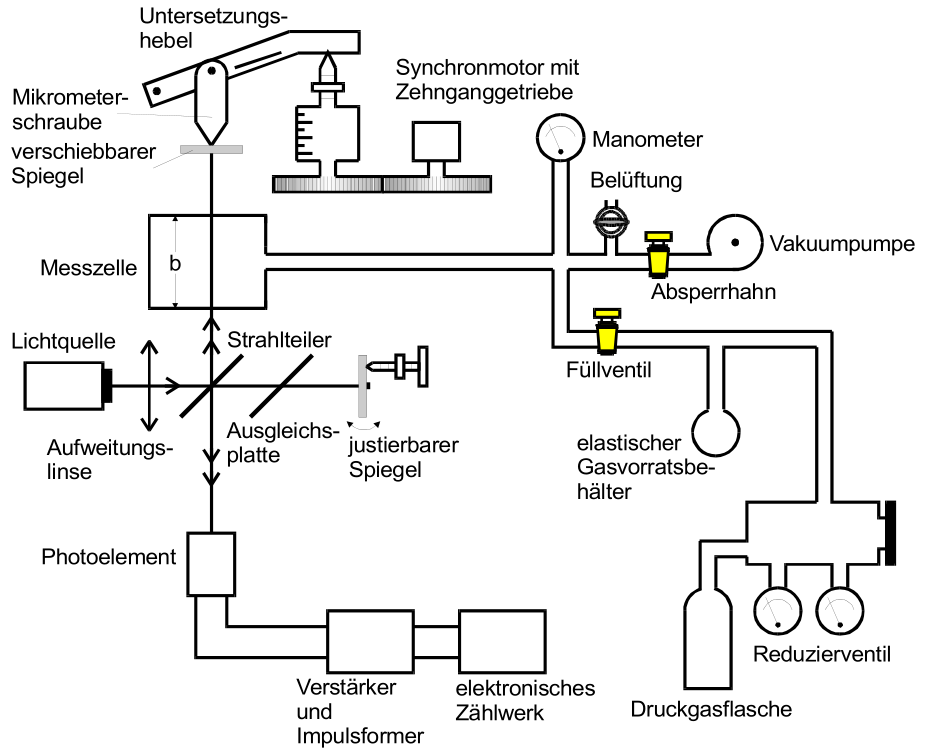
\includegraphics[width=0.9\textwidth]{latex/images/MessApp.PNG}
        \caption{Der schematische Aufbau der Messaperatur\protect \cite{V401}.}
        \label{img:4}
    \end{figure}

    \noindent Zusätzlich muss das Interferometer noch justiert werden, dazu wird der eine Spiegel erst grob verschoben so, dass die Maxima 
    übereinander liegen, danach wird der Spiegel noch feinjustiert um ein möglichst klares Interfernzmuster zu erzeugen. Dieses Interfernzbild 
    innerhalb des Maximums sollte nun genau in den Detektor fallen.

    \subsection{Bestimmung der Wellenlänge}

        \noindent Zur Bestimmung der Wellenlänge des Lasers wird ein Spiegel mittels einer Mikrometerschraube immer um 5mm verschoben. Um 
        sicherzustellen, dass wirklich genau 5mm vermessen wurden wird auf dem Rückweg von 5,5mm bis 0,5mm gemessen. Um die durchlaufene 
        Maxima zu zählen wird eine Photozelle welche an einem Zählelement angeschlossen ist, genutzt. Die Mikrometerschraube sollte bei 
        Messdurchläufen nur auf normaler einfacher Geschwindigkeit laufen, damit die Photozelle keine Maxima verpasst. Es werden nun 8 Messreihen 
        aufgenommen bei denen die Mikrometerschraube insgesamt 4 mal hin und zurück fährt. Dabei wird jeweils die Anzahl der Maxima abgelsen und 
        zurückgesetzt. Aus diesen Werten lässt sich nun die Wellenlänge des Lasers berechnen.

    \subsection{Bestimmung des Brechungsindex von Luft}

        \noindent Für die Bestimmung des Brechungsindeces von Luft wird die Versuchsaufbau nicht geändert, jetzt wird jedoch nicht mehr die Position 
        des Spiegels geändert, sonder der Druck innerhalb einer mit Luft gefüllten Messkammer. Es werden also wieder die durchlaufenen Maxima 
        gezählt während durch eine per Hand betriebene Vakuumpumpe der Druck innerhalb der Messkammer um 600 mmHg ändert. Auch hier werden 
        die Maxima beim reduzieren des Drucks und beim wiederherstellen des Drucks gemessen. Hierbei ist zu beachten, dass die Messungen während 
        die Apperatur unter Druck steht, relativ schnell abgelesen werden um Fehler durch undichte Stellen zu minimieren. Diese Messung 
        wird insgesamt 5 mal wiederholt.


